% Options for packages loaded elsewhere
\PassOptionsToPackage{unicode}{hyperref}
\PassOptionsToPackage{hyphens}{url}
%
\documentclass[
]{article}
\usepackage{amsmath,amssymb}
\usepackage{lmodern}
\usepackage{ifxetex,ifluatex}
\ifnum 0\ifxetex 1\fi\ifluatex 1\fi=0 % if pdftex
  \usepackage[T1]{fontenc}
  \usepackage[utf8]{inputenc}
  \usepackage{textcomp} % provide euro and other symbols
\else % if luatex or xetex
  \usepackage{unicode-math}
  \defaultfontfeatures{Scale=MatchLowercase}
  \defaultfontfeatures[\rmfamily]{Ligatures=TeX,Scale=1}
\fi
% Use upquote if available, for straight quotes in verbatim environments
\IfFileExists{upquote.sty}{\usepackage{upquote}}{}
\IfFileExists{microtype.sty}{% use microtype if available
  \usepackage[]{microtype}
  \UseMicrotypeSet[protrusion]{basicmath} % disable protrusion for tt fonts
}{}
\makeatletter
\@ifundefined{KOMAClassName}{% if non-KOMA class
  \IfFileExists{parskip.sty}{%
    \usepackage{parskip}
  }{% else
    \setlength{\parindent}{0pt}
    \setlength{\parskip}{6pt plus 2pt minus 1pt}}
}{% if KOMA class
  \KOMAoptions{parskip=half}}
\makeatother
\usepackage{xcolor}
\IfFileExists{xurl.sty}{\usepackage{xurl}}{} % add URL line breaks if available
\IfFileExists{bookmark.sty}{\usepackage{bookmark}}{\usepackage{hyperref}}
\hypersetup{
  pdftitle={Free Speech},
  pdfauthor={Juanshu Wu},
  hidelinks,
  pdfcreator={LaTeX via pandoc}}
\urlstyle{same} % disable monospaced font for URLs
\usepackage[margin=1in]{geometry}
\usepackage{color}
\usepackage{fancyvrb}
\newcommand{\VerbBar}{|}
\newcommand{\VERB}{\Verb[commandchars=\\\{\}]}
\DefineVerbatimEnvironment{Highlighting}{Verbatim}{commandchars=\\\{\}}
% Add ',fontsize=\small' for more characters per line
\usepackage{framed}
\definecolor{shadecolor}{RGB}{248,248,248}
\newenvironment{Shaded}{\begin{snugshade}}{\end{snugshade}}
\newcommand{\AlertTok}[1]{\textcolor[rgb]{0.94,0.16,0.16}{#1}}
\newcommand{\AnnotationTok}[1]{\textcolor[rgb]{0.56,0.35,0.01}{\textbf{\textit{#1}}}}
\newcommand{\AttributeTok}[1]{\textcolor[rgb]{0.77,0.63,0.00}{#1}}
\newcommand{\BaseNTok}[1]{\textcolor[rgb]{0.00,0.00,0.81}{#1}}
\newcommand{\BuiltInTok}[1]{#1}
\newcommand{\CharTok}[1]{\textcolor[rgb]{0.31,0.60,0.02}{#1}}
\newcommand{\CommentTok}[1]{\textcolor[rgb]{0.56,0.35,0.01}{\textit{#1}}}
\newcommand{\CommentVarTok}[1]{\textcolor[rgb]{0.56,0.35,0.01}{\textbf{\textit{#1}}}}
\newcommand{\ConstantTok}[1]{\textcolor[rgb]{0.00,0.00,0.00}{#1}}
\newcommand{\ControlFlowTok}[1]{\textcolor[rgb]{0.13,0.29,0.53}{\textbf{#1}}}
\newcommand{\DataTypeTok}[1]{\textcolor[rgb]{0.13,0.29,0.53}{#1}}
\newcommand{\DecValTok}[1]{\textcolor[rgb]{0.00,0.00,0.81}{#1}}
\newcommand{\DocumentationTok}[1]{\textcolor[rgb]{0.56,0.35,0.01}{\textbf{\textit{#1}}}}
\newcommand{\ErrorTok}[1]{\textcolor[rgb]{0.64,0.00,0.00}{\textbf{#1}}}
\newcommand{\ExtensionTok}[1]{#1}
\newcommand{\FloatTok}[1]{\textcolor[rgb]{0.00,0.00,0.81}{#1}}
\newcommand{\FunctionTok}[1]{\textcolor[rgb]{0.00,0.00,0.00}{#1}}
\newcommand{\ImportTok}[1]{#1}
\newcommand{\InformationTok}[1]{\textcolor[rgb]{0.56,0.35,0.01}{\textbf{\textit{#1}}}}
\newcommand{\KeywordTok}[1]{\textcolor[rgb]{0.13,0.29,0.53}{\textbf{#1}}}
\newcommand{\NormalTok}[1]{#1}
\newcommand{\OperatorTok}[1]{\textcolor[rgb]{0.81,0.36,0.00}{\textbf{#1}}}
\newcommand{\OtherTok}[1]{\textcolor[rgb]{0.56,0.35,0.01}{#1}}
\newcommand{\PreprocessorTok}[1]{\textcolor[rgb]{0.56,0.35,0.01}{\textit{#1}}}
\newcommand{\RegionMarkerTok}[1]{#1}
\newcommand{\SpecialCharTok}[1]{\textcolor[rgb]{0.00,0.00,0.00}{#1}}
\newcommand{\SpecialStringTok}[1]{\textcolor[rgb]{0.31,0.60,0.02}{#1}}
\newcommand{\StringTok}[1]{\textcolor[rgb]{0.31,0.60,0.02}{#1}}
\newcommand{\VariableTok}[1]{\textcolor[rgb]{0.00,0.00,0.00}{#1}}
\newcommand{\VerbatimStringTok}[1]{\textcolor[rgb]{0.31,0.60,0.02}{#1}}
\newcommand{\WarningTok}[1]{\textcolor[rgb]{0.56,0.35,0.01}{\textbf{\textit{#1}}}}
\usepackage{graphicx}
\makeatletter
\def\maxwidth{\ifdim\Gin@nat@width>\linewidth\linewidth\else\Gin@nat@width\fi}
\def\maxheight{\ifdim\Gin@nat@height>\textheight\textheight\else\Gin@nat@height\fi}
\makeatother
% Scale images if necessary, so that they will not overflow the page
% margins by default, and it is still possible to overwrite the defaults
% using explicit options in \includegraphics[width, height, ...]{}
\setkeys{Gin}{width=\maxwidth,height=\maxheight,keepaspectratio}
% Set default figure placement to htbp
\makeatletter
\def\fps@figure{htbp}
\makeatother
\setlength{\emergencystretch}{3em} % prevent overfull lines
\providecommand{\tightlist}{%
  \setlength{\itemsep}{0pt}\setlength{\parskip}{0pt}}
\setcounter{secnumdepth}{-\maxdimen} % remove section numbering
\ifluatex
  \usepackage{selnolig}  % disable illegal ligatures
\fi

\title{Free Speech}
\author{Juanshu Wu}
\date{7/9/2021}

\begin{document}
\maketitle

\#Load data and delete data who failed to consent or failed the
attention check

\begin{Shaded}
\begin{Highlighting}[]
\CommentTok{\#Load data}
\FunctionTok{library}\NormalTok{(tidyverse)}
\NormalTok{Dat }\OtherTok{\textless{}{-}} \FunctionTok{read.csv}\NormalTok{(}\StringTok{"FreeSpeech.csv"}\NormalTok{,}\ConstantTok{TRUE}\NormalTok{)}
\CommentTok{\#Only keep participants who consent to participate}
\NormalTok{Dat1 }\OtherTok{\textless{}{-}}\NormalTok{ Dat }\SpecialCharTok{\%\textgreater{}\%} \FunctionTok{filter}\NormalTok{(Consent }\SpecialCharTok{==} \StringTok{"1"}\NormalTok{) }
\CommentTok{\#Delete the participants\textquotesingle{} data that fail the attention checks}
\NormalTok{Dat\_attention\_check\_passed }\OtherTok{\textless{}{-}}\NormalTok{ Dat1 }\SpecialCharTok{\%\textgreater{}\%} \FunctionTok{filter}\NormalTok{(Attention1 }\SpecialCharTok{==} \DecValTok{1}\NormalTok{)}
\end{Highlighting}
\end{Shaded}

\#Categorize people into left and right slant

\begin{Shaded}
\begin{Highlighting}[]
\NormalTok{Dat\_filtered }\OtherTok{\textless{}{-}}\NormalTok{ Dat\_attention\_check\_passed }\SpecialCharTok{\%\textgreater{}\%} \FunctionTok{filter}\NormalTok{( Ideology }\SpecialCharTok{!=} \DecValTok{9} \SpecialCharTok{|}\NormalTok{ PoliticalParty}\SpecialCharTok{!=} \DecValTok{9}\NormalTok{)}
\NormalTok{Dat\_filtered }\OtherTok{\textless{}{-}}\NormalTok{ Dat\_filtered }\SpecialCharTok{\%\textgreater{}\%} \FunctionTok{mutate}\NormalTok{(}\AttributeTok{politicalslant =}\NormalTok{ Ideology}\SpecialCharTok{+}\NormalTok{PoliticalParty)}
\NormalTok{Dat\_filtered }\OtherTok{\textless{}{-}}\NormalTok{ Dat\_filtered }\SpecialCharTok{\%\textgreater{}\%} \FunctionTok{filter}\NormalTok{(politicalslant }\SpecialCharTok{!=} \DecValTok{0}\NormalTok{)}
\NormalTok{Dat\_filtered}\SpecialCharTok{$}\NormalTok{Political\_Slant}\OtherTok{\textless{}{-}}\FunctionTok{ifelse}\NormalTok{(Dat\_filtered}\SpecialCharTok{$}\NormalTok{politicalslant }\SpecialCharTok{\textgreater{}} \DecValTok{0}\NormalTok{,}\StringTok{"right"}\NormalTok{,}\StringTok{"left"}\NormalTok{)}
\end{Highlighting}
\end{Shaded}

\#Recode values

\begin{Shaded}
\begin{Highlighting}[]
\NormalTok{Dat\_filtered}\SpecialCharTok{$}\NormalTok{X1.Prohibited }\OtherTok{=} \FunctionTok{recode\_factor}\NormalTok{(Dat\_filtered}\SpecialCharTok{$}\NormalTok{X1.Prohibited,}\StringTok{"1"}\OtherTok{=} \StringTok{"Yes"}\NormalTok{,}\StringTok{"2"} \OtherTok{=} \StringTok{"No"}\NormalTok{,}\StringTok{"3"} \OtherTok{=} \StringTok{"Not Sure"}\NormalTok{)}
\NormalTok{Dat\_filtered}\SpecialCharTok{$}\NormalTok{X1.StudentAllow }\OtherTok{=} \FunctionTok{recode\_factor}\NormalTok{(Dat\_filtered}\SpecialCharTok{$}\NormalTok{X1.StudentAllow,}\StringTok{"1"}\OtherTok{=} \StringTok{"Yes"}\NormalTok{,}\StringTok{"2"} \OtherTok{=} \StringTok{"No"}\NormalTok{,}\StringTok{"3"} \OtherTok{=} \StringTok{"Not Sure"}\NormalTok{)}
\NormalTok{Dat\_filtered}\SpecialCharTok{$}\NormalTok{X1.FacultyAllow }\OtherTok{=} \FunctionTok{recode\_factor}\NormalTok{(Dat\_filtered}\SpecialCharTok{$}\NormalTok{X1.FacultyAllow,}\StringTok{"1"}\OtherTok{=} \StringTok{"Yes"}\NormalTok{,}\StringTok{"2"} \OtherTok{=} \StringTok{"No"}\NormalTok{,}\StringTok{"3"} \OtherTok{=} \StringTok{"Not Sure"}\NormalTok{)}
\NormalTok{Dat\_filtered}\SpecialCharTok{$}\NormalTok{X1.LibraryAllow}\OtherTok{=} \FunctionTok{recode\_factor}\NormalTok{(Dat\_filtered}\SpecialCharTok{$}\NormalTok{X1.LibraryAllow,}\StringTok{"1"}\OtherTok{=} \StringTok{"Yes"}\NormalTok{,}\StringTok{"2"} \OtherTok{=} \StringTok{"No"}\NormalTok{,}\StringTok{"3"} \OtherTok{=} \StringTok{"Not Sure"}\NormalTok{)}
\NormalTok{Dat\_filtered}\SpecialCharTok{$}\NormalTok{X2.Prohibited }\OtherTok{=} \FunctionTok{recode\_factor}\NormalTok{(Dat\_filtered}\SpecialCharTok{$}\NormalTok{X2.Prohibited,}\StringTok{"1"}\OtherTok{=} \StringTok{"Yes"}\NormalTok{,}\StringTok{"2"} \OtherTok{=} \StringTok{"No"}\NormalTok{,}\StringTok{"3"} \OtherTok{=} \StringTok{"Not Sure"}\NormalTok{)}
\NormalTok{Dat\_filtered}\SpecialCharTok{$}\NormalTok{X2.StudentAllow }\OtherTok{=} \FunctionTok{recode\_factor}\NormalTok{(Dat\_filtered}\SpecialCharTok{$}\NormalTok{X2.StudentAllow,}\StringTok{"1"}\OtherTok{=} \StringTok{"Yes"}\NormalTok{,}\StringTok{"2"} \OtherTok{=} \StringTok{"No"}\NormalTok{,}\StringTok{"3"} \OtherTok{=} \StringTok{"Not Sure"}\NormalTok{)}
\NormalTok{Dat\_filtered}\SpecialCharTok{$}\NormalTok{X2.FacultyAllow }\OtherTok{=} \FunctionTok{recode\_factor}\NormalTok{(Dat\_filtered}\SpecialCharTok{$}\NormalTok{X2.FacultyAllow,}\StringTok{"1"}\OtherTok{=} \StringTok{"Yes"}\NormalTok{,}\StringTok{"2"} \OtherTok{=} \StringTok{"No"}\NormalTok{,}\StringTok{"3"} \OtherTok{=} \StringTok{"Not Sure"}\NormalTok{)}
\NormalTok{Dat\_filtered}\SpecialCharTok{$}\NormalTok{X2.LibraryAllow}\OtherTok{=} \FunctionTok{recode\_factor}\NormalTok{(Dat\_filtered}\SpecialCharTok{$}\NormalTok{X2.LibraryAllow,}\StringTok{"1"}\OtherTok{=} \StringTok{"Yes"}\NormalTok{,}\StringTok{"2"} \OtherTok{=} \StringTok{"No"}\NormalTok{,}\StringTok{"3"} \OtherTok{=} \StringTok{"Not Sure"}\NormalTok{)}
\end{Highlighting}
\end{Shaded}

\#Plots

\#StudentAllow Proportion for most harmful belief

\begin{Shaded}
\begin{Highlighting}[]
\CommentTok{\# stacked}
\FunctionTok{ggplot}\NormalTok{(Dat\_filtered, }\FunctionTok{aes}\NormalTok{(Political\_Slant, }\AttributeTok{fill=}\NormalTok{X1.StudentAllow)) }\SpecialCharTok{+} 
  \FunctionTok{geom\_bar}\NormalTok{(}\AttributeTok{position=}\StringTok{"fill"}\NormalTok{)}\SpecialCharTok{+}\FunctionTok{theme}\NormalTok{ (}\AttributeTok{plot.title =} \FunctionTok{element\_text}\NormalTok{(}\AttributeTok{hjust =} \FloatTok{0.5}\NormalTok{),}\AttributeTok{text =} \FunctionTok{element\_text}\NormalTok{(}\AttributeTok{family =} \StringTok{"serif"}\NormalTok{, }\AttributeTok{size =} \DecValTok{12}\NormalTok{),}\AttributeTok{panel.grid.major =} \FunctionTok{element\_blank}\NormalTok{(), }\AttributeTok{panel.grid.minor =} \FunctionTok{element\_blank}\NormalTok{(),}\AttributeTok{panel.background =} \FunctionTok{element\_blank}\NormalTok{(), }\AttributeTok{axis.line =} \FunctionTok{element\_line}\NormalTok{(}\AttributeTok{colour =} \StringTok{"black"}\NormalTok{))}\SpecialCharTok{+}
\FunctionTok{ggtitle}\NormalTok{(}\StringTok{" (1) a student allowed by their university to publicly express this belief "}\NormalTok{)}\SpecialCharTok{+}\FunctionTok{labs}\NormalTok{(}\AttributeTok{y =} \StringTok{"Proportion"}\NormalTok{, }\AttributeTok{x =} \StringTok{"Political Slant"}\NormalTok{,}\AttributeTok{fill =} \StringTok{"Answer choice"}\NormalTok{)}
\end{Highlighting}
\end{Shaded}

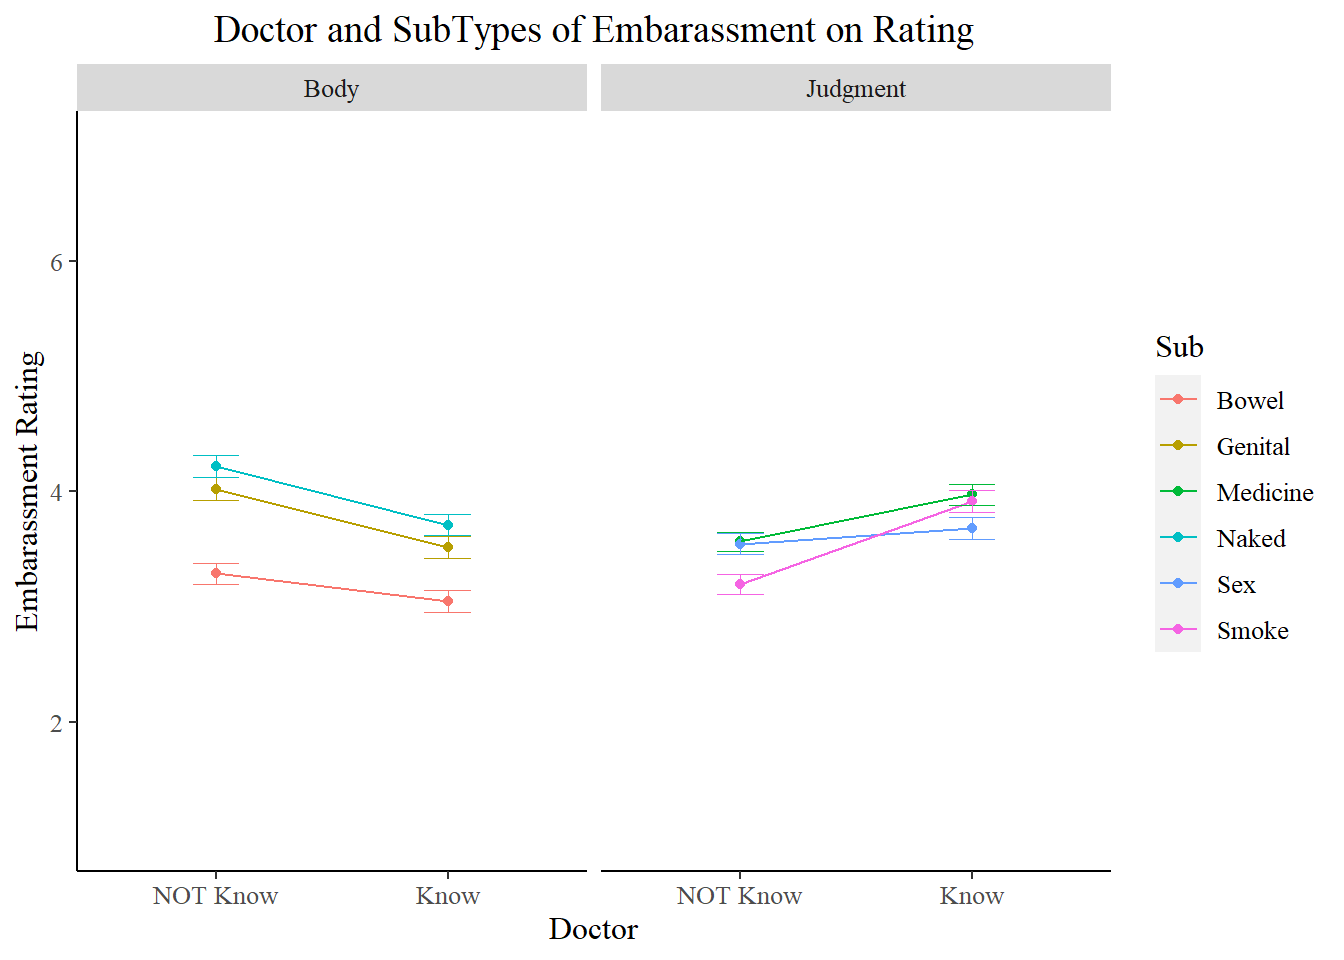
\includegraphics{FreesSpeech_files/figure-latex/unnamed-chunk-4-1.pdf}

\begin{Shaded}
\begin{Highlighting}[]
\CommentTok{\# bar dodged}
\CommentTok{\#ggplot(Dat\_filtered, aes(Political\_Slant, fill=X1.StudentAllow)) + }
  \CommentTok{\#geom\_bar(position="dodge")}
\end{Highlighting}
\end{Shaded}

\#Prohibited proportion for most harmful belief

\begin{Shaded}
\begin{Highlighting}[]
\CommentTok{\# stacked}
\FunctionTok{ggplot}\NormalTok{(Dat\_filtered, }\FunctionTok{aes}\NormalTok{(Political\_Slant, }\AttributeTok{fill=}\NormalTok{X1.Prohibited)) }\SpecialCharTok{+} 
  \FunctionTok{geom\_bar}\NormalTok{(}\AttributeTok{position=}\StringTok{"fill"}\NormalTok{)}\SpecialCharTok{+}\FunctionTok{theme}\NormalTok{(}\AttributeTok{plot.title =} \FunctionTok{element\_text}\NormalTok{(}\AttributeTok{hjust =} \FloatTok{0.5}\NormalTok{),}\AttributeTok{text =} \FunctionTok{element\_text}\NormalTok{(}\AttributeTok{family =} \StringTok{"serif"}\NormalTok{,}\AttributeTok{size =} \DecValTok{12}\NormalTok{),}\AttributeTok{panel.grid.major =} \FunctionTok{element\_blank}\NormalTok{(), }\AttributeTok{panel.grid.minor =}\FunctionTok{element\_blank}\NormalTok{(),}\AttributeTok{panel.background =} \FunctionTok{element\_blank}\NormalTok{(), }\AttributeTok{axis.line =} \FunctionTok{element\_line}\NormalTok{(}\AttributeTok{colour =} \StringTok{"black"}\NormalTok{))}\SpecialCharTok{+}
\FunctionTok{ggtitle}\NormalTok{(}\StringTok{"(1)Prohibited in US for people to express this belief publicly?"}\NormalTok{)}\SpecialCharTok{+}\FunctionTok{labs}\NormalTok{(}\AttributeTok{y =} \StringTok{"Proportion"}\NormalTok{, }\AttributeTok{x =} \StringTok{"Political Slant"}\NormalTok{,}\AttributeTok{fill =} \StringTok{"Answer choice"}\NormalTok{)}
\end{Highlighting}
\end{Shaded}

\includegraphics{FreesSpeech_files/figure-latex/unnamed-chunk-5-1.pdf}

\begin{Shaded}
\begin{Highlighting}[]
\CommentTok{\# bar dodged}
\CommentTok{\#ggplot(Dat\_filtered, aes(Political\_Slant, fill=X1.StudentAllow)) + }
  \CommentTok{\#geom\_bar(position="dodge")}
\end{Highlighting}
\end{Shaded}

\#FacultyAllow proportion for most harmful belief

\begin{Shaded}
\begin{Highlighting}[]
\CommentTok{\# stacked}
\FunctionTok{ggplot}\NormalTok{(Dat\_filtered, }\FunctionTok{aes}\NormalTok{(Political\_Slant, }\AttributeTok{fill=}\NormalTok{X1.FacultyAllow)) }\SpecialCharTok{+} 
  \FunctionTok{geom\_bar}\NormalTok{(}\AttributeTok{position=}\StringTok{"fill"}\NormalTok{)}\SpecialCharTok{+}\FunctionTok{theme}\NormalTok{(}\AttributeTok{plot.title =} \FunctionTok{element\_text}\NormalTok{(}\AttributeTok{hjust =} \FloatTok{0.5}\NormalTok{),}\AttributeTok{text =} \FunctionTok{element\_text}\NormalTok{(}\AttributeTok{family =} \StringTok{"serif"}\NormalTok{,}\AttributeTok{size =} \DecValTok{12}\NormalTok{),}\AttributeTok{panel.grid.major =} \FunctionTok{element\_blank}\NormalTok{(), }\AttributeTok{panel.grid.minor =}\FunctionTok{element\_blank}\NormalTok{(),}\AttributeTok{panel.background =} \FunctionTok{element\_blank}\NormalTok{(), }\AttributeTok{axis.line =} \FunctionTok{element\_line}\NormalTok{(}\AttributeTok{colour =} \StringTok{"black"}\NormalTok{))}\SpecialCharTok{+}
\FunctionTok{ggtitle}\NormalTok{(}\StringTok{"(1)Allow faculty member in University to express this belief publicly?"}\NormalTok{)}\SpecialCharTok{+}\FunctionTok{labs}\NormalTok{(}\AttributeTok{y =} \StringTok{"Proportion"}\NormalTok{, }\AttributeTok{x =} \StringTok{"Political Slant"}\NormalTok{,}\AttributeTok{fill =} \StringTok{"Answer choice"}\NormalTok{)}
\end{Highlighting}
\end{Shaded}

\includegraphics{FreesSpeech_files/figure-latex/unnamed-chunk-6-1.pdf}

\begin{Shaded}
\begin{Highlighting}[]
\CommentTok{\# bar dodged}
\CommentTok{\#ggplot(Dat\_filtered, aes(Political\_Slant, fill=X1.StudentAllow)) + }
  \CommentTok{\#geom\_bar(position="dodge")}
\end{Highlighting}
\end{Shaded}

\#Library allow porpotion for most harmful belief

\begin{Shaded}
\begin{Highlighting}[]
\CommentTok{\# stacked}
\FunctionTok{ggplot}\NormalTok{(Dat\_filtered, }\FunctionTok{aes}\NormalTok{(Political\_Slant, }\AttributeTok{fill=}\NormalTok{X1.LibraryAllow)) }\SpecialCharTok{+} 
  \FunctionTok{geom\_bar}\NormalTok{(}\AttributeTok{position=}\StringTok{"fill"}\NormalTok{)}\SpecialCharTok{+}\FunctionTok{theme}\NormalTok{(}\AttributeTok{plot.title =} \FunctionTok{element\_text}\NormalTok{(}\AttributeTok{hjust =} \FloatTok{0.5}\NormalTok{),}\AttributeTok{text =} \FunctionTok{element\_text}\NormalTok{(}\AttributeTok{family =} \StringTok{"serif"}\NormalTok{,}\AttributeTok{size =} \DecValTok{12}\NormalTok{),}\AttributeTok{panel.grid.major =} \FunctionTok{element\_blank}\NormalTok{(), }\AttributeTok{panel.grid.minor =}\FunctionTok{element\_blank}\NormalTok{(),}\AttributeTok{panel.background =} \FunctionTok{element\_blank}\NormalTok{(), }\AttributeTok{axis.line =} \FunctionTok{element\_line}\NormalTok{(}\AttributeTok{colour =} \StringTok{"black"}\NormalTok{))}\SpecialCharTok{+}
\FunctionTok{ggtitle}\NormalTok{(}\StringTok{"(1)library should ban this belief?"}\NormalTok{)}\SpecialCharTok{+}\FunctionTok{labs}\NormalTok{(}\AttributeTok{y =} \StringTok{"Proportion"}\NormalTok{, }\AttributeTok{x =} \StringTok{"Political Slant"}\NormalTok{,}\AttributeTok{fill =} \StringTok{"Answer choice"}\NormalTok{)}
\end{Highlighting}
\end{Shaded}

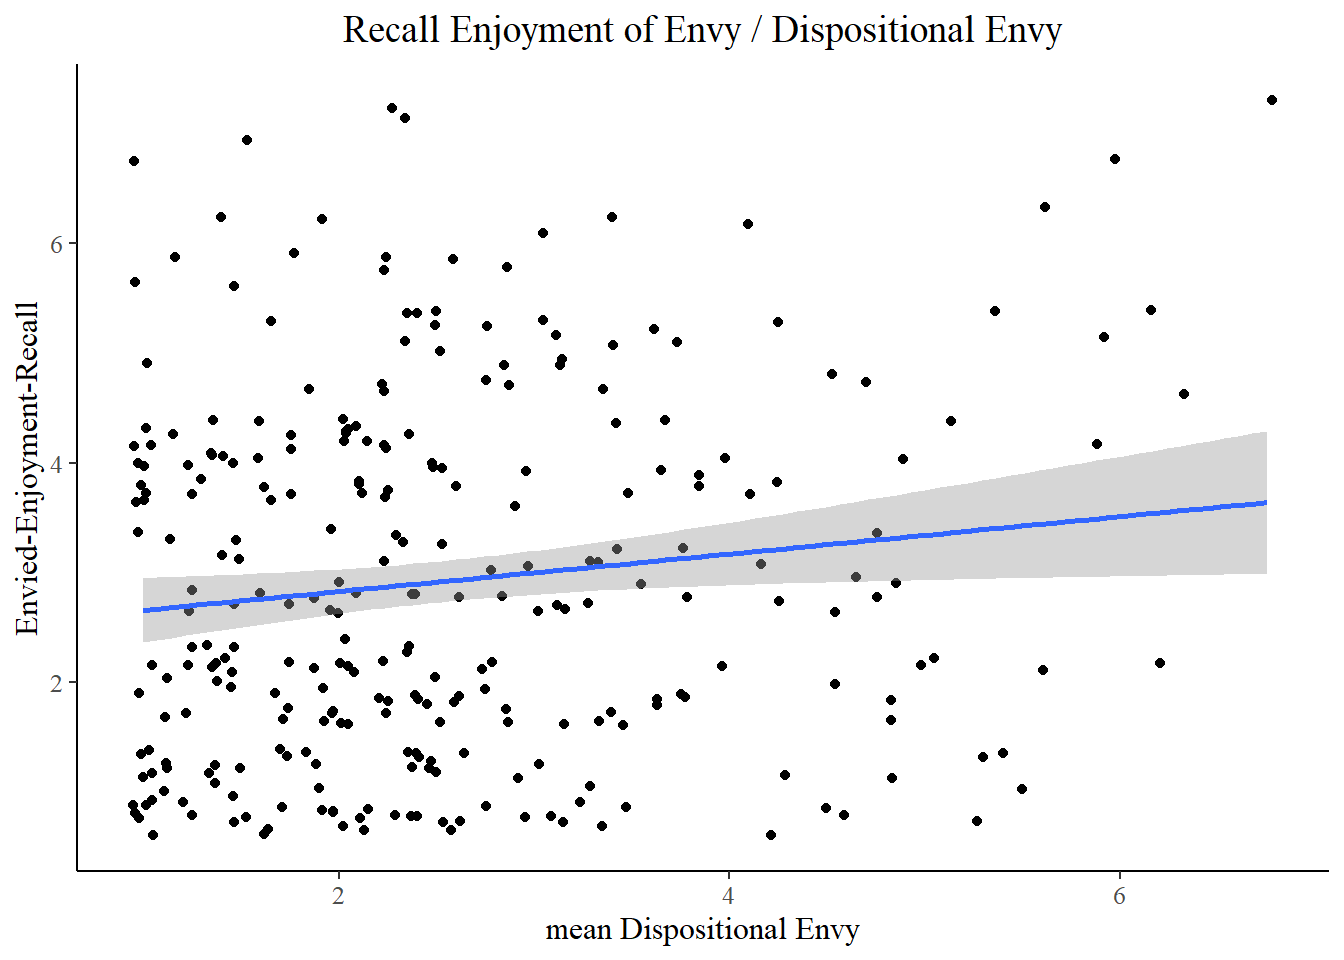
\includegraphics{FreesSpeech_files/figure-latex/unnamed-chunk-7-1.pdf}

\begin{Shaded}
\begin{Highlighting}[]
\CommentTok{\# bar dodged}
\CommentTok{\#ggplot(Dat\_filtered, aes(Political\_Slant, fill=X1.StudentAllow)) + }
  \CommentTok{\#geom\_bar(position="dodge")}
\end{Highlighting}
\end{Shaded}

\#Student Allow proportion for second most harmful belief

\begin{Shaded}
\begin{Highlighting}[]
\CommentTok{\# stacked}
\FunctionTok{ggplot}\NormalTok{(Dat\_filtered, }\FunctionTok{aes}\NormalTok{(Political\_Slant, }\AttributeTok{fill=}\NormalTok{X2.StudentAllow)) }\SpecialCharTok{+} 
  \FunctionTok{geom\_bar}\NormalTok{(}\AttributeTok{position=}\StringTok{"fill"}\NormalTok{)}\SpecialCharTok{+}\FunctionTok{theme}\NormalTok{ (}\AttributeTok{plot.title =} \FunctionTok{element\_text}\NormalTok{(}\AttributeTok{hjust =} \FloatTok{0.5}\NormalTok{),}\AttributeTok{text =} \FunctionTok{element\_text}\NormalTok{(}\AttributeTok{family =} \StringTok{"serif"}\NormalTok{, }\AttributeTok{size =} \DecValTok{12}\NormalTok{),}\AttributeTok{panel.grid.major =} \FunctionTok{element\_blank}\NormalTok{(), }\AttributeTok{panel.grid.minor =} \FunctionTok{element\_blank}\NormalTok{(),}\AttributeTok{panel.background =} \FunctionTok{element\_blank}\NormalTok{(), }\AttributeTok{axis.line =} \FunctionTok{element\_line}\NormalTok{(}\AttributeTok{colour =} \StringTok{"black"}\NormalTok{))}\SpecialCharTok{+}\FunctionTok{ggtitle}\NormalTok{(}\StringTok{"(2) a student allowed by their university to publicly express this belief"}\NormalTok{)}\SpecialCharTok{+}\FunctionTok{labs}\NormalTok{(}\AttributeTok{y =}\StringTok{"Proportion"}\NormalTok{, }\AttributeTok{x =} \StringTok{"Political Slant"}\NormalTok{,}\AttributeTok{fill =} \StringTok{"Answer choice"}\NormalTok{)}
\end{Highlighting}
\end{Shaded}

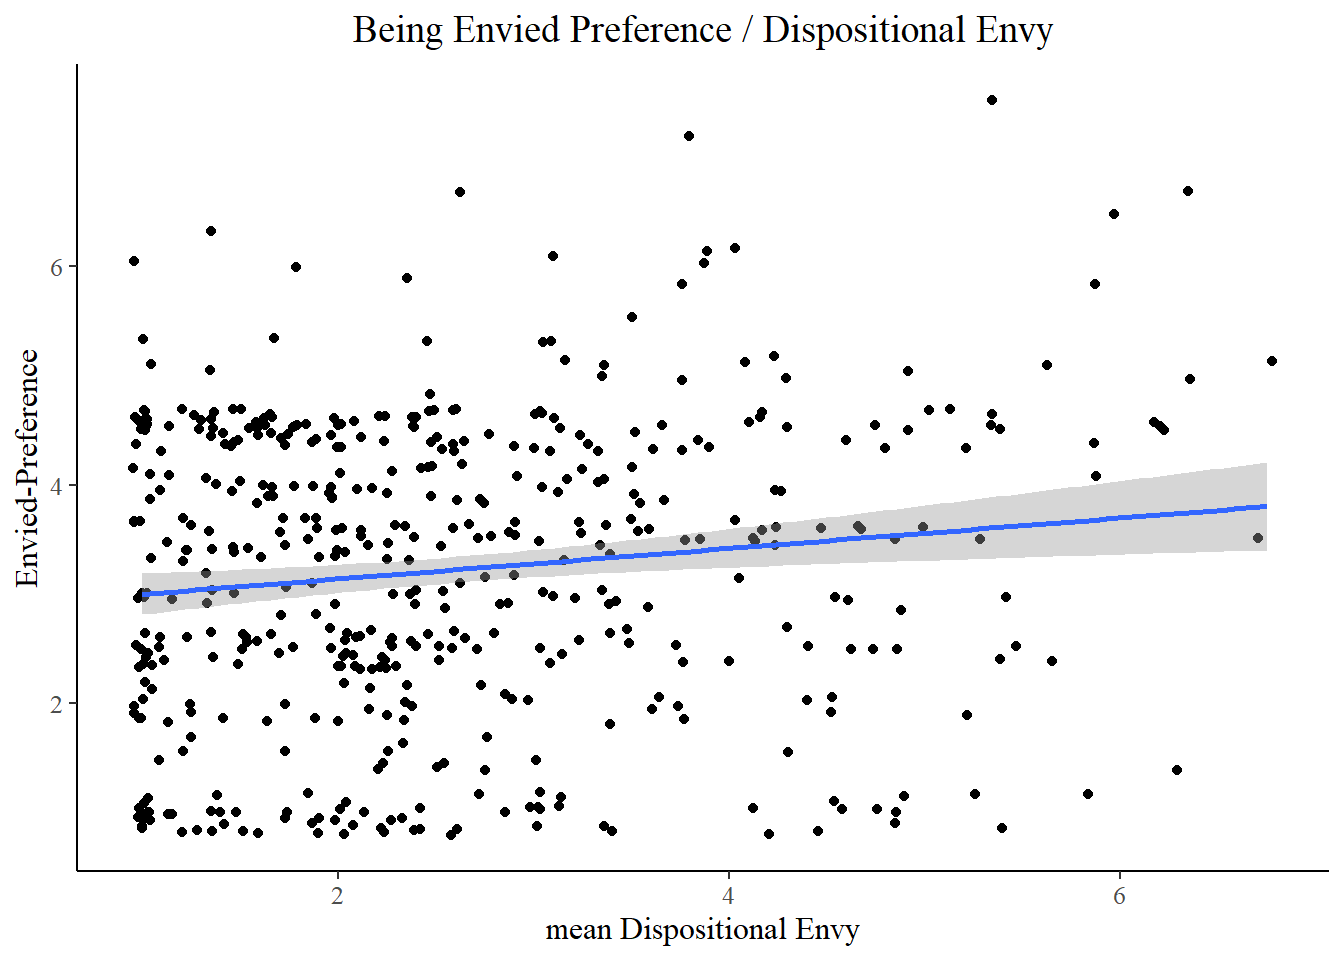
\includegraphics{FreesSpeech_files/figure-latex/unnamed-chunk-8-1.pdf}

\begin{Shaded}
\begin{Highlighting}[]
\CommentTok{\# bar dodged}
\CommentTok{\#ggplot(Dat\_filtered, aes(Political\_Slant, fill=X1.StudentAllow)) + }
  \CommentTok{\#geom\_bar(position="dodge")}
\end{Highlighting}
\end{Shaded}

\#Prohibited proprotion for second most harmful belief

\begin{Shaded}
\begin{Highlighting}[]
\CommentTok{\# stacked}
\FunctionTok{ggplot}\NormalTok{(Dat\_filtered, }\FunctionTok{aes}\NormalTok{(Political\_Slant, }\AttributeTok{fill=}\NormalTok{X2.Prohibited)) }\SpecialCharTok{+} 
  \FunctionTok{geom\_bar}\NormalTok{(}\AttributeTok{position=}\StringTok{"fill"}\NormalTok{)}\SpecialCharTok{+}\FunctionTok{theme}\NormalTok{(}\AttributeTok{plot.title =} \FunctionTok{element\_text}\NormalTok{(}\AttributeTok{hjust =} \FloatTok{0.5}\NormalTok{),}\AttributeTok{text =} \FunctionTok{element\_text}\NormalTok{(}\AttributeTok{family =} \StringTok{"serif"}\NormalTok{,}\AttributeTok{size =} \DecValTok{12}\NormalTok{),}\AttributeTok{panel.grid.major =} \FunctionTok{element\_blank}\NormalTok{(), }\AttributeTok{panel.grid.minor =}\FunctionTok{element\_blank}\NormalTok{(),}\AttributeTok{panel.background =} \FunctionTok{element\_blank}\NormalTok{(), }\AttributeTok{axis.line =} \FunctionTok{element\_line}\NormalTok{(}\AttributeTok{colour =} \StringTok{"black"}\NormalTok{))}\SpecialCharTok{+}
\FunctionTok{ggtitle}\NormalTok{(}\StringTok{"(2)Prohibited in US for people to express this belief publicly?"}\NormalTok{)}\SpecialCharTok{+}\FunctionTok{labs}\NormalTok{(}\AttributeTok{y =} \StringTok{"Proportion"}\NormalTok{, }\AttributeTok{x =} \StringTok{"Political Slant"}\NormalTok{,}\AttributeTok{fill =} \StringTok{"Answer choice"}\NormalTok{)}
\end{Highlighting}
\end{Shaded}

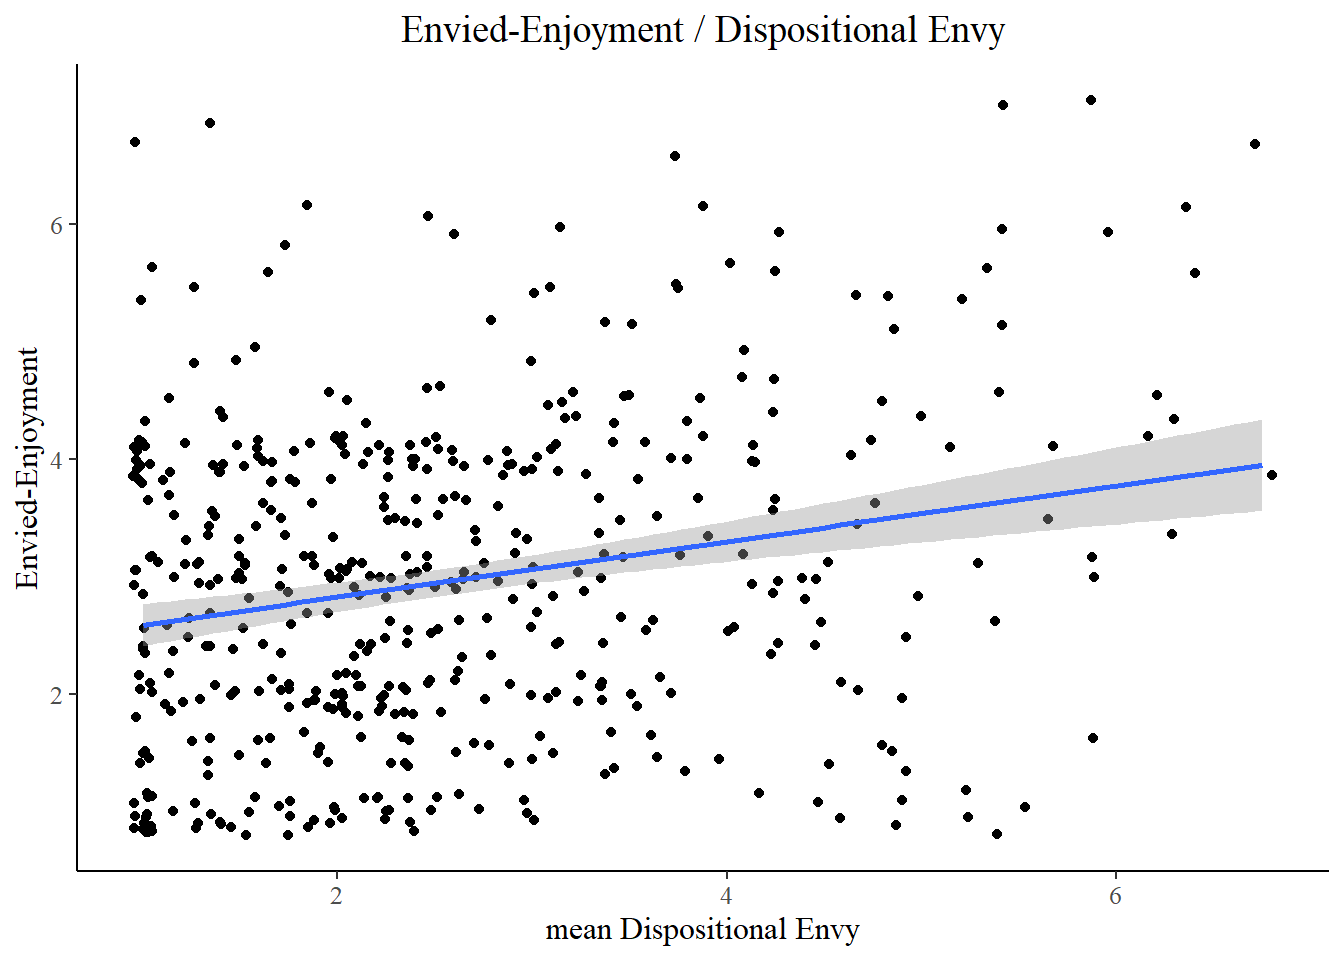
\includegraphics{FreesSpeech_files/figure-latex/unnamed-chunk-9-1.pdf}

\begin{Shaded}
\begin{Highlighting}[]
\CommentTok{\# bar dodged}
\CommentTok{\#ggplot(Dat\_filtered, aes(Political\_Slant, fill=X1.StudentAllow)) + }
  \CommentTok{\#geom\_bar(position="dodge")}
\end{Highlighting}
\end{Shaded}

\#FacultyAllow proportion for second most harmful belief

\begin{Shaded}
\begin{Highlighting}[]
\CommentTok{\# stacked}
\FunctionTok{ggplot}\NormalTok{(Dat\_filtered, }\FunctionTok{aes}\NormalTok{(Political\_Slant, }\AttributeTok{fill=}\NormalTok{X2.FacultyAllow)) }\SpecialCharTok{+} 
  \FunctionTok{geom\_bar}\NormalTok{(}\AttributeTok{position=}\StringTok{"fill"}\NormalTok{)}\SpecialCharTok{+}\FunctionTok{theme}\NormalTok{(}\AttributeTok{plot.title =} \FunctionTok{element\_text}\NormalTok{(}\AttributeTok{hjust =} \FloatTok{0.5}\NormalTok{),}\AttributeTok{text =} \FunctionTok{element\_text}\NormalTok{(}\AttributeTok{family =} \StringTok{"serif"}\NormalTok{,}\AttributeTok{size =} \DecValTok{12}\NormalTok{),}\AttributeTok{panel.grid.major =} \FunctionTok{element\_blank}\NormalTok{(), }\AttributeTok{panel.grid.minor =}\FunctionTok{element\_blank}\NormalTok{(),}\AttributeTok{panel.background =} \FunctionTok{element\_blank}\NormalTok{(), }\AttributeTok{axis.line =} \FunctionTok{element\_line}\NormalTok{(}\AttributeTok{colour =} \StringTok{"black"}\NormalTok{))}\SpecialCharTok{+}
\FunctionTok{ggtitle}\NormalTok{(}\StringTok{"(2)Allow faculty member in University to express this belief publicly?"}\NormalTok{)}\SpecialCharTok{+}\FunctionTok{labs}\NormalTok{(}\AttributeTok{y =} \StringTok{"Proportion"}\NormalTok{, }\AttributeTok{x =} \StringTok{"Political Slant"}\NormalTok{,}\AttributeTok{fill =} \StringTok{"Answer choice"}\NormalTok{)}
\end{Highlighting}
\end{Shaded}

\includegraphics{FreesSpeech_files/figure-latex/unnamed-chunk-10-1.pdf}

\begin{Shaded}
\begin{Highlighting}[]
\CommentTok{\# bar dodged}
\CommentTok{\#ggplot(Dat\_filtered, aes(Political\_Slant, fill=X1.StudentAllow)) + }
  \CommentTok{\#geom\_bar(position="dodge")}
\end{Highlighting}
\end{Shaded}

\#LibraryAllow proportion for second most harmful belief

\begin{Shaded}
\begin{Highlighting}[]
\CommentTok{\# stacked}
\FunctionTok{ggplot}\NormalTok{(Dat\_filtered, }\FunctionTok{aes}\NormalTok{(Political\_Slant, }\AttributeTok{fill=}\NormalTok{X2.LibraryAllow)) }\SpecialCharTok{+} 
  \FunctionTok{geom\_bar}\NormalTok{(}\AttributeTok{position=}\StringTok{"fill"}\NormalTok{)}\SpecialCharTok{+}\FunctionTok{theme}\NormalTok{(}\AttributeTok{plot.title =} \FunctionTok{element\_text}\NormalTok{(}\AttributeTok{hjust =} \FloatTok{0.5}\NormalTok{),}\AttributeTok{text =} \FunctionTok{element\_text}\NormalTok{(}\AttributeTok{family =} \StringTok{"serif"}\NormalTok{,}\AttributeTok{size =} \DecValTok{12}\NormalTok{),}\AttributeTok{panel.grid.major =} \FunctionTok{element\_blank}\NormalTok{(), }\AttributeTok{panel.grid.minor =}\FunctionTok{element\_blank}\NormalTok{(),}\AttributeTok{panel.background =} \FunctionTok{element\_blank}\NormalTok{(), }\AttributeTok{axis.line =} \FunctionTok{element\_line}\NormalTok{(}\AttributeTok{colour =} \StringTok{"black"}\NormalTok{))}\SpecialCharTok{+}
\FunctionTok{ggtitle}\NormalTok{(}\StringTok{"(2)library should ban this belief?"}\NormalTok{)}\SpecialCharTok{+}\FunctionTok{labs}\NormalTok{(}\AttributeTok{y =} \StringTok{"Proportion"}\NormalTok{, }\AttributeTok{x =} \StringTok{"Political Slant"}\NormalTok{,}\AttributeTok{fill =} \StringTok{"Answer choice"}\NormalTok{)}
\end{Highlighting}
\end{Shaded}

\includegraphics{FreesSpeech_files/figure-latex/unnamed-chunk-11-1.pdf}

\begin{Shaded}
\begin{Highlighting}[]
\CommentTok{\# bar dodged}
\CommentTok{\#ggplot(Dat\_filtered, aes(Political\_Slant, fill=X1.StudentAllow)) + }
  \CommentTok{\#geom\_bar(position="dodge")}
\end{Highlighting}
\end{Shaded}


\end{document}
